\documentclass{article}
\usepackage[utf8]{inputenc}
\pagenumbering{Roman}
\usepackage{ragged2e}
\usepackage{graphicx}
\usepackage{wrapfig}
\usepackage[spanish]{babel}
\usepackage{hyperref}
\usepackage{datetime}


\begin{document}


\title{\huge \textbf{Instructivo para la extracción de datos de monitor de signos vitales y BIS } \vspace{8cm}}
\author{Carlos Valle \\ \href{mailto:cgvalle@uc.cl}{cgvalle@uc.cl} }
\date{21 de Febrero 2024}
\maketitle


\newpage

\section{Motivación}

El objetivo de este instructivo es guiar en el setup de equipos y software para la extración de datos del monitor de signos vitales \href{https://www.gehealthcare.com/products/patient-monitoring/patient-monitors/carescape-monitor-b650}{Carescape B650} y el monitor \href{https://www.medtronic.com/covidien/es-cl/products/brain-monitoring/bis-complete-4-channel-monitor.html}{Bis vista}.

Los procedimientos para obtener los datos de ambos equipos son independientes por lo que se abordaran en dos secciones independientes. En cada sección se describirá el setup, así como el uso del software necesario. 

Los códigos y archivos necesarios se encuentran alojados en la carpeta de GitHub: \url{https://github.com/cgvalle/monitor_signos_vitales} 


\newpage



% B650
\section{Monitor Carescape B650}
Para la extracción de las señales fisiológicas durante cirugia se utiliza el monitor Carescape B650 (Fig. \ref{fig:b650_frontal}). Los códigos e instructivos se basan en dicho monitor, por lo que no se asegura la compatibilidad con un tercero. 

\begin{figure}[h]
	\centering
    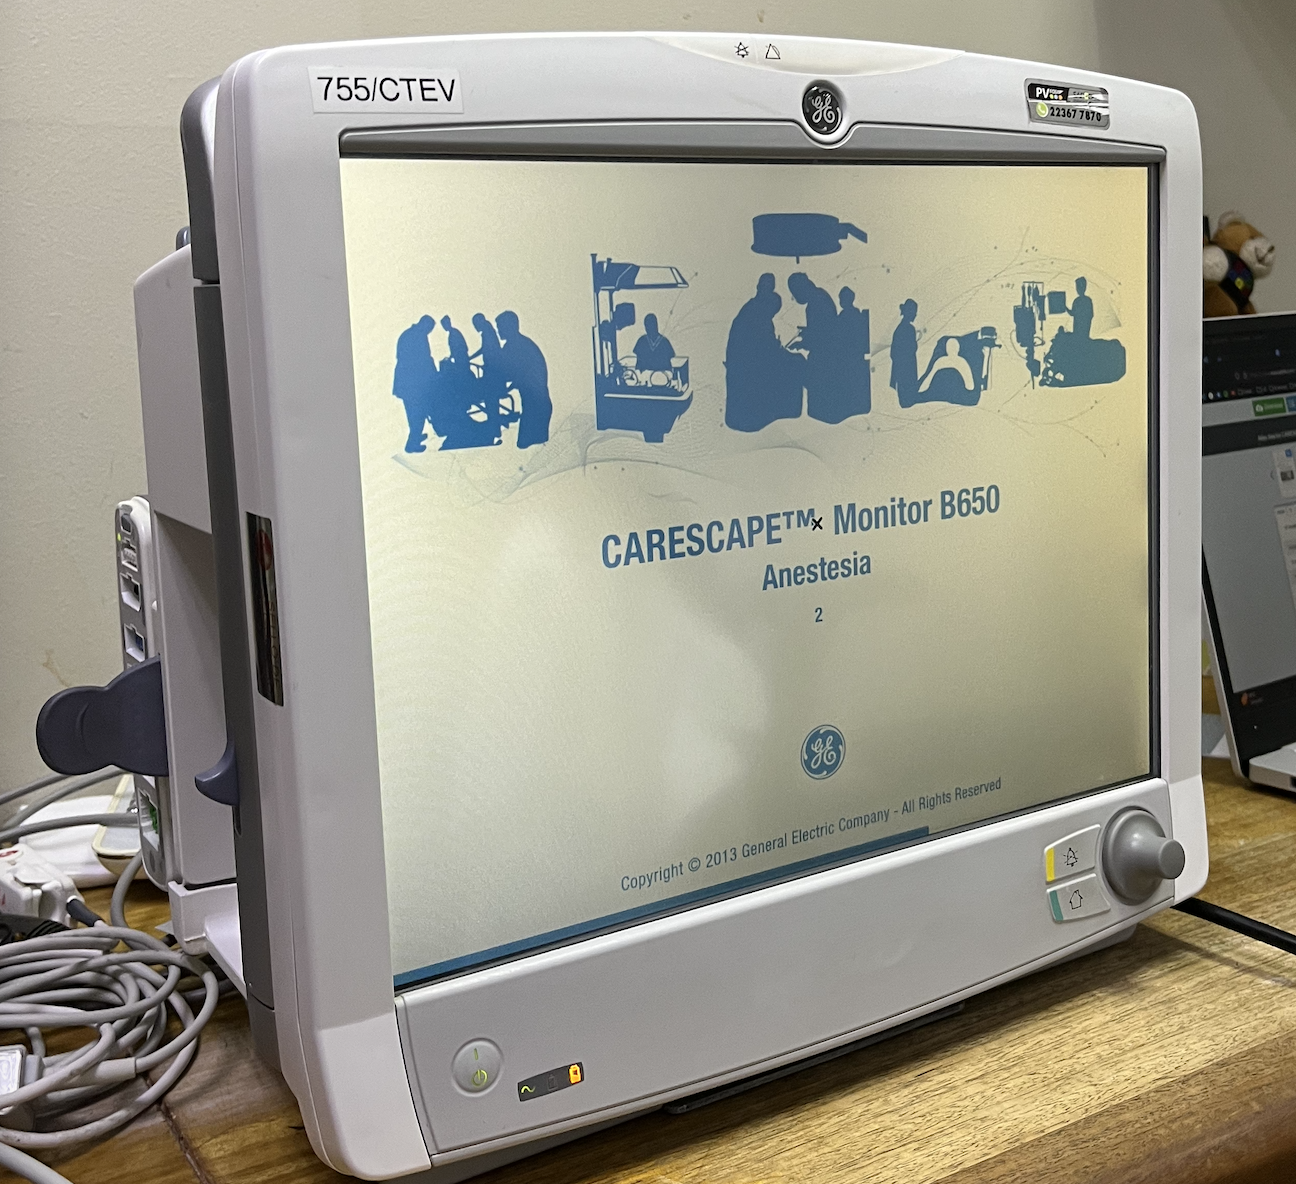
\includegraphics[scale=0.6]{img/carescape_b650.jpeg}
    \caption{Vista frontal monitor Carescape B650}
    \label{fig:b650_frontal}
\end{figure}

\subsection{Setup}
Cables necesarios:

\begin{enumerate}
	\item Cable ATEN USB to Serial RS232.  (Es necesario que cuente con el chip VID 0557, modelos mas nuevos vienen con 067b. De necesitar otro, buscarlo en ebay priorizando el más viejo que exista para aumentar las probabilidades de que venga con el chip VID 0557)

	\includegraphics*[scale=0.12]{img/ATEN_USB.jpeg}
	\item  Cable RS232 hembra hembra 

	\includegraphics*[scale=0.12]{img/rs232_hembra_hembra.jpeg}
	\item Cable RS232 a usb (Null Modem)

	\includegraphics*[scale=0.12]{img/rs232_macho_a_usb.jpeg}

\end{enumerate}










\newpage

\begin{figure}
	\centering
    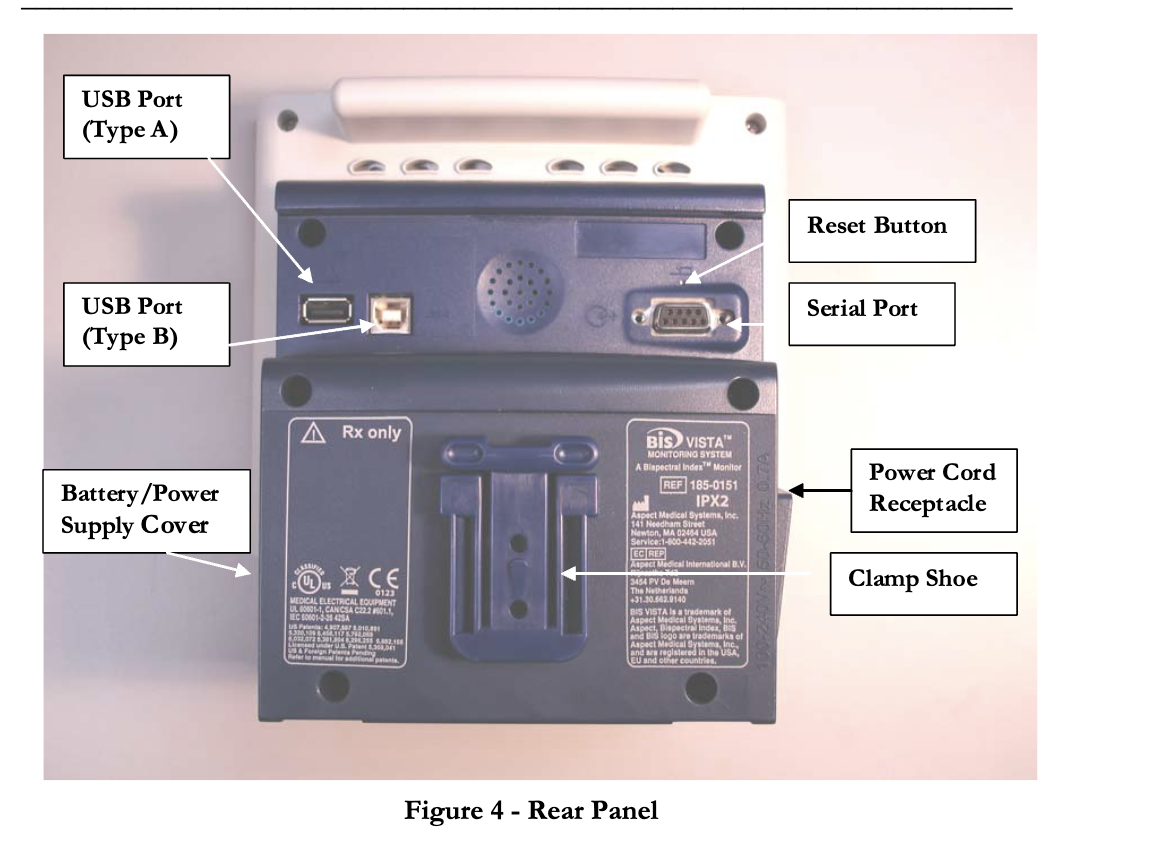
\includegraphics[scale=0.5]{img/bis_rear_panel.png}
    \caption{Caption}
\end{figure}






\end{document}
